\documentclass{article}
%\usepackage{fullpage}
\usepackage{mathtools}
\usepackage{mhchem}
\usepackage{amssymb}
\usepackage{amsmath}
\usepackage{bm}
\usepackage{gensymb}
\usepackage{siunitx}
\usepackage{cancel}
\usepackage{graphicx}
\usepackage{subcaption}
\usepackage{mdframed}
\author{Mann, J}
\title{Day X Notes}
\date{September 29, 2015}
\newenvironment{aside}{\begin{mdframed}}{\end{mdframed}}
\renewcommand{\d}[0]{\mathrm{d}}
\newcommand{\pOne}[2]{\frac{\partial #1}{\partial #2}}
\renewcommand{\deg}[0]{\degree}
\newcommand{\pTwo}[2]{\frac{\partial^2 #1}{\partial #2^2}}
\newcommand{\dOne}[2]{\frac{\d #1}{\d #2}}
\newcommand{\dTwo}[2]{\frac{\d^2 #1}{\d #2^2}}
\newcommand{\diag}[1]{\bcancel{#1}}
\newcommand{\matr}[1]{\bm{#1}}
\newcommand{\note}[1]{\vspace{3\parsep}\textit{\textbf{Note: }}#1\vspace{2\parsep}}
\newcommand{\norm}[1]{\left|#1\right|}
\newcommand{\qsubn}[0]{\vec{q}_n}
\newcommand{\xsubn}[0]{\vec{x}_n}
\newcommand{\xvec}[0]{\vec{x}}
\newcommand{\qvec}[0]{\vec{q}}
\newcommand{\aOne}[0]{\vec{a}_1}
\newcommand{\aTwo}[0]{\vec{a}_2}
\newcommand{\ein}[0]{\hat{e}_\text{in}}
\newcommand{\esc}[0]{\hat{e}_\text{sc}}

\graphicspath{{Day10NotesPics/}}
\begin{document}
\maketitle{}
\begin{section}{Foundations of a crystal surface structure}
	Tyndall effect is scattering of light in a dispersion.
	\begin{itemize}
		\item Compute $q$ for a light scattering experiment for a colloid
		\item Compute $\vec{q}_n$ for a surface net.
		\item $\aOne$, $\aTwo$ in direct space and $\aOne^\ast,\aTwo^\ast$ in reciprocal space.
		\item Cross-product method to generate $\aOne^\ast,\aTwo^\ast$ the matrix method.
		\item For next time - adsorption produces an adsorbate net on the adsorbent net.
	\end{itemize}
	There are two ways to look at things: Microscopy and scattering
\end{section}
\begin{section}{}
	\begin{figure}[h]
		\centering
		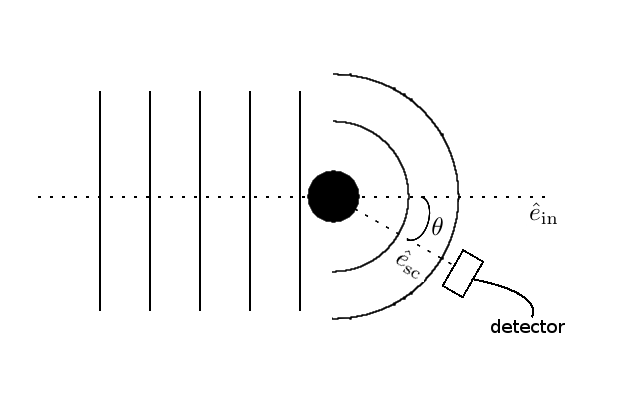
\includegraphics[height=60pt]{atomWave}
		\caption{Assume the source is a laser.}
		\label{fig:laser}
	\end{figure}

	Your retina acts as a square law detector. If you look carefully, you can see an intensity difference when viewing a solution with a light shining through at different angles.

	An electric field, $\phi$ is converted (often to a photocurrent, $i_\text{pc}$ according to 
	\begin{align*}
		\phi\ast\phi \alpha i_\text{pc}\\
		\phi = f_1 e^{\pi \vec{q}\cdot\vec{x}_1}
	\end{align*}
	$f_1$ is called the form factor, or scattering cross-section. Note that $\vec{x}_1$ is in direct space and $\vec{q}$ is in reciprocal space. Either space may be used.

	\end{section}
\begin{section}{Compute $\norm{\vec{q}}$ for $\theta_\text{scattered}$}
	You know that momentum is balanced and 
	\begin{align*}
		E_\text{in} &= E_\text{sc}
	\end{align*}
	This implies that
	\begin{align*}
		\norm{q} &= f(k,\text{etc.})\\
		k &= \frac{2\pi}{\lambda_\text{light}}\\
	\end{align*}
	The momentum balance says:
	\begin{align*}
		\vec{q} &= k(\ein-\esc)
	\end{align*}
	Now, if we define
	\begin{align*}
		\ein &= (0,0,1)\\
		\esc &= (\sin\theta\cos\phi,\sin\theta\sin\phi,\cos\theta)
	\end{align*}

	For many dispersions, you don't get additional information scanning in $\phi$, therefore we take $\phi=0$, and obtain:

	\begin{align*}
		\ein &= (0,0,1)\\
		\esc &= (\sin\theta,0,\cos\theta)\\
		\vec{q} &= \ein - \esc = k(\sin\theta,0,1-\cos\theta)\\
		\norm{q} &= \sqrt{\vec{q}\cdot\vec{q}}\\
		&= \sqrt{ k^2( \sin^2\theta + (1 - \cos\theta)^2)}\\
		&= \sqrt{ k^2(\sin^2\theta + 1 - 2\cos\theta + \cos^2\theta)}\\
		&= \sqrt{ k^2(\sin^2\theta + 2 - 2\cos\theta - 1 + \cos^2\theta)}\\
		&= \sqrt{ k^2(\sin^2\theta - (1 - \cos^2) + 2\cos\theta}\\
		&= \sqrt{ 2 k^2(2\sin^2\frac{\theta}{2})}\\
		&= \sqrt{ 4k^2\sin^2\frac{\theta}{2}}\\
		&= 2 k \sin\frac{\theta}{2}
	\end{align*}
	scatter from solution: intensity as a function of $\theta$ convert to $q$.
	\begin{align*}
		\phi = \sum_{n=0}^{N\times N}e^{i\vec{q}\cdot\vec{x}_n}
	\end{align*}
	the field for scattering from a net of $N\times N$ particles with each atom represented by $\vec{x}_n = m_1 \vec{a}_1 + m_2\vec{a}_2$ 
	$\vec{a}_1 + m_2\vec{a}_2$ are vectors in the 2-space of surface diffraction.
\end{section}
\begin{section}{}

	\begin{figure}[h]
		\centering
		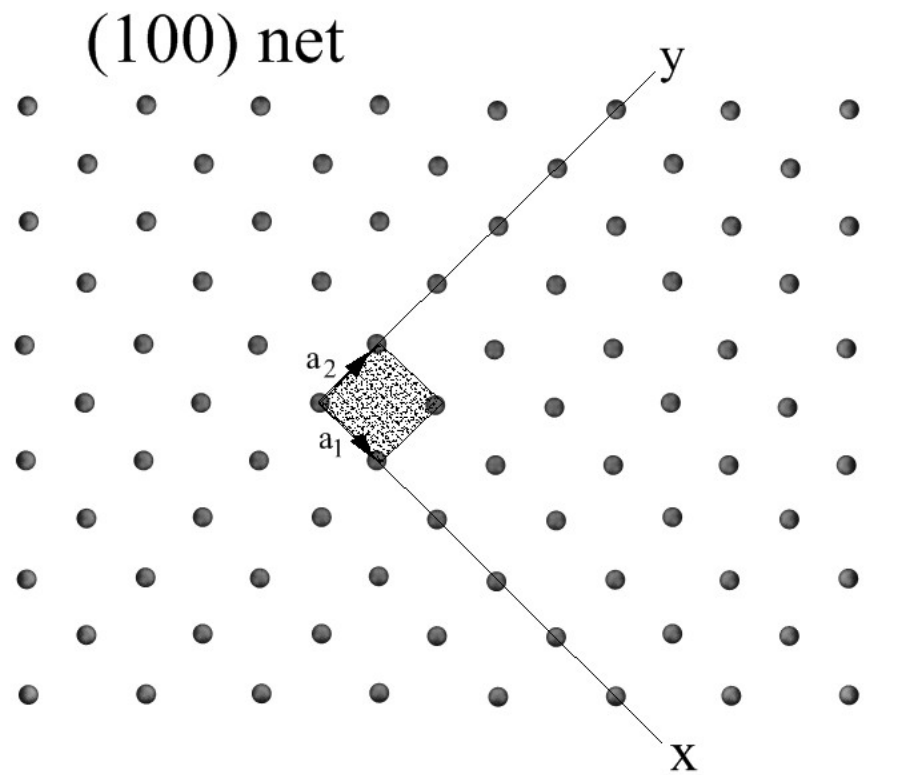
\includegraphics[height=100pt]{100plane2}
		\caption{A 2-D Lattice, or Net.}
		\label{fig:Net}
	\end{figure}
	Remember the net and think of the density $\rho(\vec{x})$

		Remember the net and think of the density $\rho(\vec{x})$
	
		Imagine that you have a really good microscope, and what you see in your microscope is a pattern like Figure~\ref{fig:Net}. Locate each atom.

		What I need is some kind of a pointer. Let's define one:
		\begin{subsection}{Dirac Delta}
		\begin{align*}
			\delta(\vec{x}-\vec{x}_n) (\text{Dirac delta function})
		\end{align*}

		\begin{figure}[h]
			\centering
			\begin{subfigure}[t]{0.4\textwidth}
				\centering
				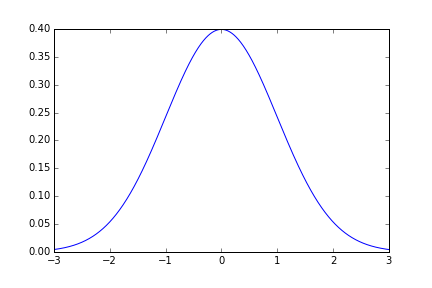
\includegraphics[height=65pt]{gaussian}
				\caption{Gaussian}
				\label{fig:Gauss}
			\end{subfigure}
			\begin{subfigure}[t]{0.4\textwidth}
				\centering
				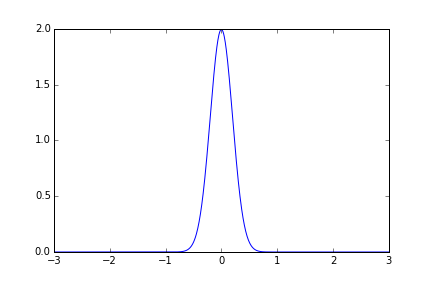
\includegraphics[height=65pt]{sharpgauss}
				\caption{Gaussian with $\sigma = \frac{1}{5}$}
				\label{fig:sharpGauss}
			\end{subfigure}
			\begin{subfigure}[t]{0.5\textwidth}
				\centering
				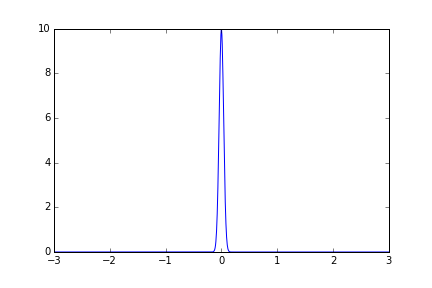
\includegraphics[height=65pt]{verysharpgauss}
				\caption{Gaussian with $\sigma = \frac{1}{25}$. This is starting to look like the dirac delta function $\delta(x)$}
				\label{fig:almostdirac}
			\end{subfigure}
			\caption{For a gaussian function $G(x,\mu=0,\sigma) = G(x,\sigma)$, the dirac delta function can be thought of as $\delta(x) = \lim\limits_{\sigma\rightarrow 0}G(x,\sigma)$}
		\end{figure}
		Suppose I have a unit step function. This is the integral of the dirac delta function. You could show this by looking at the step function and its derivative.
		\begin{align*}
			\int_{-\infty}^{+\infty}&f(x)\d(\alpha(x))\\
			\alpha(x) &= \begin{cases}0\text{ for }x<0\\1\text{ for }x>0\end{cases}\\
			\int_{-\infty}^{+\infty}f(x)\d(\alpha(x))  &\sum_{\text{partition}}f(x^\ast)(\alpha(x_{-1}-\alpha(x_{+1})))
		\end{align*}
The interval $(\alpha(x_{-1})-\alpha(x_{+1}))$ gives 1.

Limit of the partition length goes to zero.
\begin{align*}
			\int_{-\infty}^{+\infty}f(x)\d(\alpha(x)) &= f(0)\\
			\d(\alpha(x))&\rightarrow \delta(x) \d x\\
			\int_{-\infty}^{+\infty}\delta(x)\d x &= 1\\
			\int_{-\infty}^{+\infty} f(x)\delta(x) dx &= f(0)\\
			\int_{-\infty}^{+\infty}f(x)\delta(x-x_0) &= f(x_0)
\end{align*}

\end{subsection}
\begin{subsection}{Application}
Now what I do is to say that
\begin{align*}
	\rho(\vec{x}) = \sum_{n=0}^{N\times N}\delta(\vec{x}-\vec{x}_n)
\end{align*}
this is an $N$ by $N$ net of atoms. Given any $\vec{x}$ whatsoever, this will tell you what atoms are close to that $\vec{x}$

Now 
\begin{align*}
	\int_{\text{domain}}\rho(\vec{x}) \d\vec{x} &= \sum_{n=0}^{N\times N}\int_{\text{domain}}\delta(\vec{x}-\vec{x}_n)\d \vec{x}\\
	&= \text{Number of atoms in domain D.}
\end{align*}

Now suppose that I take the Fourier Transform of $\rho(\vec{x})$
\end{subsection}
\begin{subsection}{Fourier}
	\note{$\rho(\vec{x})$ is in direct space. Now go to reciprocal space by Fourier transform.}
	\begin{align*}
		\int_{-\infty}^{\infty}\rho(x)e^{i\vec{q}\xvec}\d x &= \sum_{n=0}^{N\times N}\int_{-\infty}^{+\infty}\delta(x-x_n)e^{i\vec{q}\cdot \xvec}\d x\\
		&= \sum_{n=0}^{N\times N}e^{i\vec{q}\cdot\xsubn}
	\end{align*}
	But this is exactly the result of the $\phi$ calculation.
\end{subsection}
\end{section}
\begin{section}{}
	\begin{align*}
		\hat{F}(\rho(\xvec)) = \sum_{n=0}^{N\times N}e^{i\vec{q}\cdot\xsubn}
	\end{align*}
	The representation in $\qvec$ space.

	I will get a set of delta functions in $\qvec$ space.

	Let's substitute:
	\begin{align*}
		\xsubn = m_1\aOne + m_2\aTwo
	\end{align*}

	Keep in mind that $m_1$ and $m_2$ are signed integers.

	If I take 
	\begin{align*}
		\phi = \sum_{n=0}^{N\times N}e^{i\qvec\cdot (m_1\aOne + m_2\aTwo)}
	\end{align*}
	Compute $\phi\ast \phi$. 

	First we need to show that we can write
	\begin{align*}
		\phi = \left(\sum_{m_1 = 0}^{N}e^{i\qvec\cdot(m_1\aOne)}\right)\left(\sum_{m_2 = 0}^{N}e^{i\qvec\cdot(m_2\aTwo)}\right)
	\end{align*}
	Given 
	\begin{align*}
		\phi = \sum_{n=0}^{N\times N}e^{i\qvec\cdot\xvec}
	\end{align*} 
This is true, but you should try it in the privacy of your office. Look for a pattern and see for yourself.

Result is going to be that the 
\begin{align*}
	\norm{\phi}^2 = \left(\frac{\sin{(\frac{1}{2})}N\qvec\cdot\aOne}{\sin{(\frac{1}{2})}\qvec\cdot\aOne}\right)\left(\frac{\sin{(\frac{1}{2})}N\qvec\cdot\aTwo}{\sin{(\frac{1}{2})}\qvec\cdot\aTwo}\right)
\end{align*}
\end{section}
\begin{section}{Conclusion}
	How large can you have a coherent domain in a graphene lattice? How large are the domains of the adsorbate and the adsorbent in terms of the catalytic processes? These are properties that you can calculate with this.

	What you find is, suppose that my domain is like Figure~\ref{fig:Net}, except $4\times 4$, so $N=16$. Now what you find is that the function looks something like a gaussian.

	If you choose $N=10^4$, you start to look much more like a dirac delta function.

	If the fuzzy balls look like points, then you have a small domain size. Large fuzzy balls mean large domain size. These are the diffraction patterns.
\end{section}
\end{document}
